% !TEX encoding = ISO-8859-1

Nesta sessão, serão descritos os experimentos realizados e os resultados obtidos.

\subsection{K-Means}
\label{subsec:exp-kmeans}

O K-Means, já abordado na sessão \ref{subsec:teoria-kmeans}, foi utilizado neste experimento com $K$ = 2, o que significa que ele gera 2 clusters. O algoritmo foi executado 100 vezes e foi escolhido o resultado de maior adequação entre os clusters e seus representantes.

A figura \ref{fig:clusters} mostra graficamente os clusters formados pelo K-Means.

\begin{figure}[H]
\center
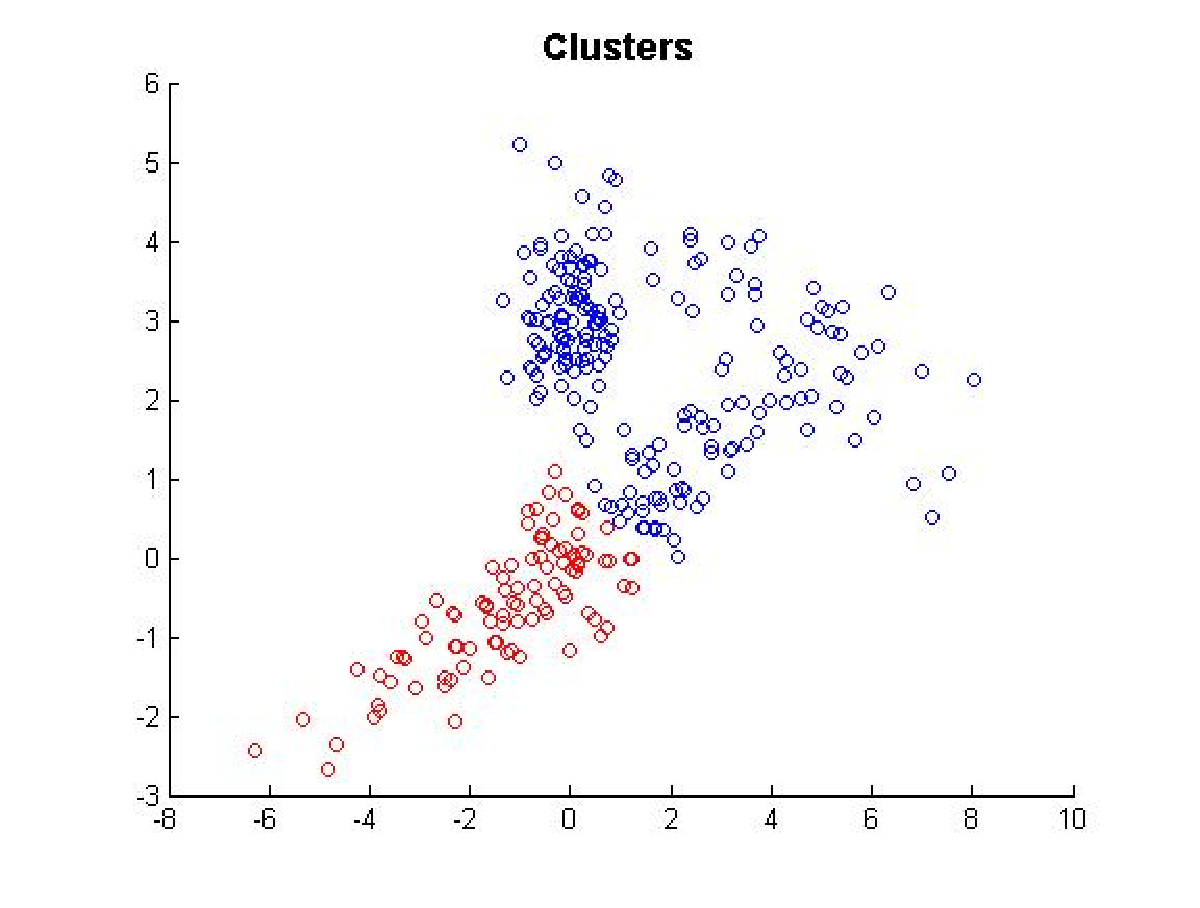
\includegraphics[scale=0.60]{imagens/tecnicas/clusters.eps}
\caption{Clusters gerados pelo K-Means}
\label{fig:clusters}
\end{figure}

Após a clusterização, é necessário associar cada cluster a uma classe. Para fazer isso, foi obtido o centroide de cada cluster e o centroide de cada classe, e foi associada a Classe 1, o cluster com centroide mais próximo do centroide da Classe 1, o cluster mais distante foi associado a Classe 2.

Para avaliar o desempenho do K-Means, foi calculada a taxa de erro de classificação global e por classe. Além disso, também foi calculado o Índice de Rand Corrigido.

\begin{table}[H]
\begin{center}
\begin{tabular}{|l|l|l|l|}
\hline
Erro Global	&	Erro da Classe 1	&	Erro da Classe 2	&	Rand Corrigido	\\
\hline %----- linha horizontal
TAXA AQUI	&		TAXA AQUI		&		TAXA AQUI		&	TAXA AQUI		\\
\hline
\end{tabular}%--- fechamento do ambiente tabular
\end{center}   %fim da centralização da tabela
\caption{Tabela da taxa de erro do K-Means}
\label{tab:erro-kmeans}
\end{table}

Os resultados obtidos estão representados na tabela \ref{tab:erro-kmeans}.


\subsection{Classificadores}
\label{subsec:exp-classificadores}

Nesta sessão, serão avaliados os resultados dos classificadores utilizando os dados já citados na sessão \ref{sec:geracaodados}. Os classificadores obedecem a regra de decisão especificada abaixo:

\begin{equation}
j = argmax_i P(\omega_{i} | x_{k},\theta{i})
\end{equation}
com
\begin{equation}
P(\omega_{i} | x_{k},\theta{i}) = \dfrac{p(x_k| \omega_i, \theta_i) \times P(\omega_i)}{\sum_{j=1}^c p(x_k | \omega_j, \theta_j) \times P(\omega_j)}
\end{equation}


\subsubsection{Máxima Verossimilhança e Algoritmo EM}
\label{subsubsec:exp-mle-em}

Nesta subsessão, as estimativas de $P(\omega_i | x_k, \theta_i)$ foram feitas de formas diferentes para as duas classes. Para Classe 1, foi utilizado o Método da Máxima Verossimilhança, supondo uma normal multivariada. Já para a Classe 2, classe que possui 2 conjuntos diferentes (ver sessão \ref{sec:geracaodados}), foi utilizado o algoritmo EM, supondo a existencia de 2 componentes e uma mistura de distribuições normais multivaridas.

Inicialmente, o conjunto de dados foi dividido em Treino e Teste, esta divisão foi feita utilizando a proporção 30\% para teste e 70\% para treino.

Para a Classe 1, obteve-se as instâncias de treinamento desta classe e foram obtidas as médias e o desvio padrão de cada atributo desta classe. Com as médias e o desvio padrão, foi utilizada a função do MATLAB $mvnpdf$, passando como parâmetro as instâncias de teste, a média e o desvio padrão das instâncias de treinamento da Classe 1. Assim, obteve-se a \textit{pdf} da Classe 1.

Já para a Classe 2, por se tratar de uma distribuição multimodal, foi utilizada a função do MATLAB $gmdistribution.fit$, passando como argumentos as instâncias de treinamento da Classe 2 e a quantidade de componentes, no caso 2. Então, obteve-se os parâmetros necessários para utilizar a função $mvnpdf$ para se obter a primeira e a segunda distribuição normal.

Porém, para ainda é necessário associar cada \textit{pdf} da Classe 2 a sua respectiva componente, para isso, utilizou-se a média de cada sub-conjunto em relação as médias utilizadas para construir as \textit{pdfs}. Assim, é feita a proporção, utilizando a quantidade de instâncias nos sub-conjuntos das classes, para estimar a \textit{pdf} resultante da Classe 2.

Por fim, com as \textit{pdfs} de cada classe, para cada instância, caso a probabilidade a posteriori da Classe 1 for maior ou igual que a da Classe 2, a instância é classificada como sendo da Classe 1, caso contrário, é classificada como sendo da Classe 2.

Os resultados estão descritos na tabela abaixo:

\begin{table}[H]
\begin{center}
\begin{tabular}{|l|l|l|l|}
\hline
Erro Global	&	Erro da Classe 1	&	Erro da Classe 2	&	Rand Corrigido	\\
\hline %----- linha horizontal
TAXA AQUI	&		TAXA AQUI		&		TAXA AQUI		&	TAXA AQUI		\\
\hline
\end{tabular}%--- fechamento do ambiente tabular
\end{center}   %fim da centralização da tabela
\caption{Tabela da taxa de erro do MLE e EM combinados}
\label{tab:erro-mle-em}
\end{table}

\subsubsection{Janela de Parzen}
\label{subsubsec:exp-janeladeparzen}









